%%%%%%%%%%%%%%%%%%%%%%%%%%%%%%%%%%%%%%%%%%%%%%%%%%%%%%%%%%%%%%%%%%%%%
% LaTeX Template: Project Titlepage Modified (v 0.1) by rcx
%
% Original Source: http://www.howtotex.com
% Date: February 2014
% 
% This is a title page template which be used for articles & reports.
% 
% This is the modified version of the original Latex template from
% aforementioned website.
% 
%%%%%%%%%%%%%%%%%%%%%%%%%%%%%%%%%%%%%%%%%%%%%%%%%%%%%%%%%%%%%%%%%%%%%%

\documentclass[12pt]{report}
\usepackage[a4paper]{geometry}
\usepackage[myheadings]{fullpage}
\usepackage{fancyhdr}
\usepackage{lastpage}
\usepackage{graphicx, wrapfig, subcaption, setspace, booktabs}
\usepackage[T1]{fontenc}
\usepackage[font=small, labelfont=bf]{caption}
% \usepackage{fourier}
\usepackage[protrusion=true, expansion=true]{microtype}
\usepackage[english]{babel}
\usepackage{sectsty}
\usepackage{url, lipsum}


\newcommand{\HRule}[1]{\rule{\linewidth}{#1}}
\onehalfspacing
\setcounter{tocdepth}{5}
\setcounter{secnumdepth}{5}

%-------------------------------------------------------------------------------
% HEADER & FOOTER
%-------------------------------------------------------------------------------
\pagestyle{fancy}
\fancyhf{}
\renewcommand{\footrulewidth}{0.4pt}
\setlength\headheight{15pt}
\fancyhead[L]{Project Report}
\fancyhead[R]{EE-331L Electric Machines Lab}
\fancyfoot[R]{Page \thepage\ of \pageref{LastPage}}
%-------------------------------------------------------------------------------
% TITLE PAGE
%-------------------------------------------------------------------------------

\begin{document}

\title{ \normalsize \textsc{EE-331L Electric Machines Lab}
		\\ [2.0cm]
		\HRule{0.5pt} \\
		\LARGE \textbf{\uppercase{Simulation of Smart Grid in Simulink}}
		\HRule{2pt} \\ [0.5cm]
		\normalsize \today \vspace*{5\baselineskip}}

\date{}

\author{
		Minhaj Ahmed Moin - hm02896 \\ 
		Ahmed Bilal Arsal - ba00315 \\
		Habib University \\}

\maketitle

\begin{abstract}
    Power distribution is carried out from the grid station through transmission lines. The electricity generated in the power station through various methods such as hydro-electric generation, nuclear power plant, wind turbines and so on and so forth. Previously, the advent of synchronous generators enabled us to produce electricity via methods mentioned above. However, there has always been a continuous need for innovation due to the growing population and also due to environmental changes i.e. global warming. Thus, not only the need for innovation allowed the engineers to come with new ideas of producing better efficient methods of generating electricity but also has digitized a lot of processes involved in achieving the finished product. One of the key methods is the simulation of the raw products in order o test them before their implementation in real time which is a cost effective method and saves resources as well.This project aims to simulate the working of the smart grid using MATLAB SIMULINK.
\end{abstract}

% \tableofcontents
% \newpage

%-------------------------------------------------------------------------------
% Section title formatting
% \sectionfont{\scshape}
%-------------------------------------------------------------------------------

%-------------------------------------------------------------------------------
% BODY
%-------------------------------------------------------------------------------

\section*{Introduction}

Smart Grids allow for two way communication between homes and power plants. This exchange may be in the form of electricity or digital signals. Electricity as exchange medium is used when a Consumer has a renewable energy source like Solar Panels directly connected to it. The main grid and the renewable energy Source provide the energy required for the consumer's needs, if the energy source is unable to fulfill the requirements by itself. If it can, then the grid's electricity is not used by the consumer but instead it can supply the excess energy from the source to the grid. In this way, a two way exchange can be set up.The other case, which is implemented through this project is when information is exchanged both ways between the houses or the loads and the grid or the power generation site. Through this method, important parameters such as load consumption can be monitored remotely from the power generation site and changes to the grid can be made accordingly. This is also known as supervisory control and data acquisition, or simply, SCADA. 

\section*{Rationale of the Model}
In this Project, we have model a simulation of smart grid with Solar Cells i.e. Photo voltaic cells which is a modern method of power generation and is renewable energy source as well. DC current and voltages are output by the photo voltaic cells. This DC is converted to AC via a DC to AC converter which outputs three phase voltages 120 degrees out of phase.Block of three phase voltages and current measurements are used along with scopes to verify the output at different instants in the schematic . The line losses have been modelled by using a three phase pi section line and loads have been connected with circuit breakers to the grid network.Furthermore, two more Photo voltaic arrays have been implemented in the schematic and are connected to it using circuit breakers. The Breakers connecting the loads to the grid are programmed to close the circuit at 2 and 3.5 seconds respectively. Using a comparator the second and third sources are activated when the required power exceeds the supplied power of the PV arrays. In this way an efficient method of management of PV arrays to produce electricity as per demand on the distribution side is carried out and resources are managed properly without any wastage.


\section*{Discussion on the Design Issues}
The main design issue in the making of this project was the implementation of PV arrays and connecting them to the circuit. This is because the PV arrays require us to satisfy five different equations along with several other parameters. Furthermore, an actual smart grid simulation essentially requires a maximum power point tracking algorithm which is implemented in PV inverters and continuously adjusts the impedance seen by the solar array to keep the PV system operating at the peak power point of the PV panel under varying conditions, like changing solar irradiance, temperature, and load. However, the implementation of MPPT also was beyond the scope of this project due to limited knowledge on the use of simlink and several additional parameters that are required along with the PV array equations therefore a sample has been taken for simulation purpose. Another important issue was that of power consumption and the implementation of the feedback system consisting of the comparators and control system for closing of the circuit breakers. The connected loads are programmed to consume 750 Watts of Power. The Breakers were to close at specified times. This issue could be solved by monitoring the RMS Value of the Active Power Consumption in the Loads. This power level was fed into the comparator which would give the signal to whether activate the next source or not. Following are the the equations and parameters for the PV array, and also the P\&O algorithm diagram:
\begin{center}
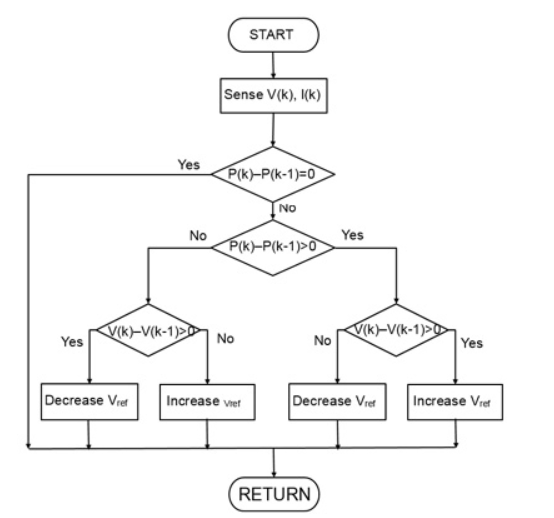
\includegraphics[scale=0.8]{pics/1.PNG}
\end{center}
\begin{center}
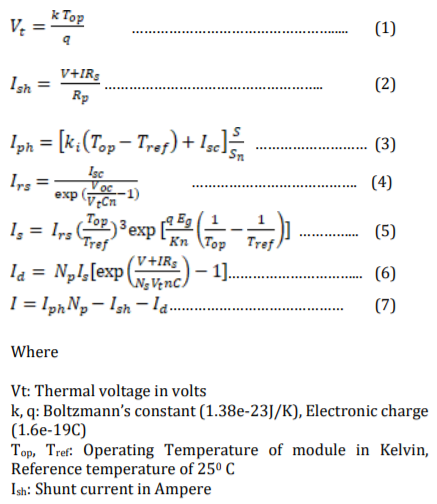
\includegraphics[scale=0.8]{pics/2.PNG}
\end{center}
\begin{center}
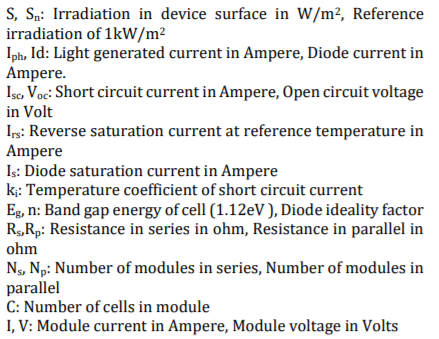
\includegraphics[scale=0.8]{pics/3.PNG}
\end{center}

\section*{Conclusion}

This simulation project is for resistive loads of an ideal smart grid System. However, in real time,  this may not be the case since there are inductive and capacitive loads as well. That essentially requires change the design of the schematic but it can very well be used as a foundation to build up on it.\\


---------------------------------------REFERENCES-------------------------------------------

Sandeep Neupane, \& Ajay Kumar. (07 July -2017). Modeling and Simulation of PV array in Matlab/Simulink for comparison of perturb and observe \& incremental conductance algorithms using buck converter. Volume 4.
\end{document}

%-------------------------------------------------------------------------------
% SNIPPETS
%-------------------------------------------------------------------------------

%\begin{figure}[!ht]
%	\centering
%	\includegraphics[width=0.8\textwidth]{file_name}
%	\caption{}
%	\centering
%	\label{label:file_name}
%\end{figure}

%\begin{figure}[!ht]
%	\centering
%	\includegraphics[width=0.8\textwidth]{graph}
%	\caption{Blood pressure ranges and associated level of hypertension (American Heart Association, 2013).}
%	\centering
%	\label{label:graph}
%\end{figure}

%\begin{wrapfigure}{r}{0.30\textwidth}
%	\vspace{-40pt}
%	\begin{center}
%		\includegraphics[width=0.29\textwidth]{file_name}
%	\end{center}
%	\vspace{-20pt}
%	\caption{}
%	\label{label:file_name}
%\end{wrapfigure}

%\begin{wrapfigure}{r}{0.45\textwidth}
%	\begin{center}
%		\includegraphics[width=0.29\textwidth]{manometer}
%	\end{center}
%	\caption{Aneroid sphygmomanometer with stethoscope (Medicalexpo, 2012).}
%	\label{label:manometer}
%\end{wrapfigure}

%\begin{table}[!ht]\footnotesize
%	\centering
%	\begin{tabular}{cccccc}
%	\toprule
%	\multicolumn{2}{c} {Pearson's correlation test} & \multicolumn{4}{c} {Independent t-test} \\
%	\midrule	
%	\multicolumn{2}{c} {Gender} & \multicolumn{2}{c} {Activity level} & \multicolumn{2}{c} {Gender} \\
%	\midrule
%	Males & Females & 1st level & 6th level & Males & Females \\
%	\midrule
%	\multicolumn{2}{c} {BMI vs. SP} & \multicolumn{2}{c} {Systolic pressure} & \multicolumn{2}{c} {Systolic Pressure} \\
%	\multicolumn{2}{c} {BMI vs. DP} & \multicolumn{2}{c} {Diastolic pressure} & \multicolumn{2}{c} {Diastolic pressure} \\
%	\multicolumn{2}{c} {BMI vs. MAP} & \multicolumn{2}{c} {MAP} & \multicolumn{2}{c} {MAP} \\
%	\multicolumn{2}{c} {W:H ratio vs. SP} & \multicolumn{2}{c} {BMI} & \multicolumn{2}{c} {BMI} \\
%	\multicolumn{2}{c} {W:H ratio vs. DP} & \multicolumn{2}{c} {W:H ratio} & \multicolumn{2}{c} {W:H ratio} \\
%	\multicolumn{2}{c} {W:H ratio vs. MAP} & \multicolumn{2}{c} {\% Body fat} & \multicolumn{2}{c} {\% Body fat} \\
%	\multicolumn{2}{c} {} & \multicolumn{2}{c} {Height} & \multicolumn{2}{c} {Height} \\
%	\multicolumn{2}{c} {} & \multicolumn{2}{c} {Weight} & \multicolumn{2}{c} {Weight} \\
%	\multicolumn{2}{c} {} & \multicolumn{2}{c} {Heart rate} & \multicolumn{2}{c} {Heart rate} \\
%	\bottomrule
%	\end{tabular}
%	\caption{Parameters that were analysed and related statistical test performed for current study. BMI - body mass index; SP - systolic pressure; DP - diastolic pressure; MAP - mean arterial pressure; W:H ratio - waist to hip ratio.}
%	\label{label:tests}
%\end{table}